\chapter{Regulatory}

\section{PID}

Ponieważ regulator PID to jest regulator o jednym wejściu i jednym wyjściu, w danym przypadku możemy użyć maksymalnie trzech regulatorów PID, jako że liczba wyjść procesu jest równa 3. Patrząc na odpowiedzi skokowe możemy ocenić które wejście ma największy wpływ na które wyjście i dla takich par $u - y$ nastroić regulatory PID. Na jedno wejście procesu w takim podejściu ustawiamy stałą.

\medskip

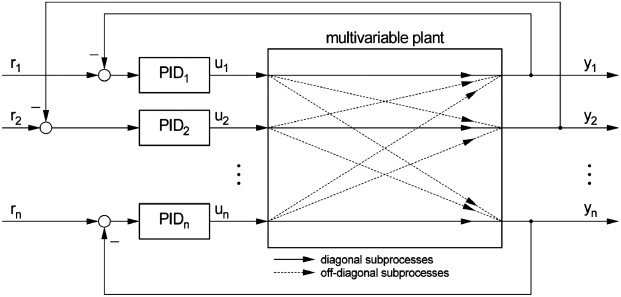
\includegraphics{../images/MPID.jpg}

\section{DMC}

Regulator DMC z natury jest wielowymiarowy. Prawo regulacji wielowymiarowego DMC w wersji klasycznej wygląda następująco:

\begin{math}
    \Delta U(k) = K(Y^{zad}(k) - Y^0(k))
\end{math}

Wektor przyrostów sterowania wynacza przyrosty na całym horyzoncie sterowania i ma długośś $n_uN_U$.

\begin{math}
    \Delta U(k) = \begin{bmatrix}
        \Delta u_1(k|k) \\
        \vdots  \\
        \Delta u_{n_u}(k|k) \\
        \vdots  \\
        \vdots  \\
        \Delta u_{1}(k + N_u - 1|k) \\
        \vdots  \\
        \Delta u_{n_u}(k + N_u - 1|k) \\
    \end{bmatrix}
\end{math}

Wektory $Y^{zad}(k)$ i $Y(k)$ są wektorami wyjść i wyjść zadanych o długości $n_yN$.

\begin{math}
    Y^{zad}(k) = \begin{bmatrix}
        y^{zad}_1(k) \\
        \vdots \\
        y^{zad}_{n_y}(k) \\
        \vdots \\
        \vdots \\
        y^{zad}_1(k) \\
        \vdots \\
        y^{zad}_{n_y}(k) \\
    \end{bmatrix}
\end{math}

\begin{math}
    Y(k) = \begin{bmatrix}
        y_1(k) \\
        \vdots \\
        y_{n_y}(k) \\
        \vdots \\
        \vdots \\
        y_1(k) \\
        \vdots \\
        y_{n_y}(k) \\
    \end{bmatrix}
\end{math}

$K$ jest macierzą następującą:

\begin{math}
    K = (M^T \varPsi M + \varLambda )^{-1} M^T \varPsi 
\end{math}

$Y^0$ jest wektorem wyjść modelu.

\begin{math}
    Y^0(k) = Y(k) + M^p \Delta U^p(k)
\end{math}

W którym $\Delta U^p(k)$ jest wektorem przeszłych przyrostów, natomiast $M^p$:

\begin{math}
    M^p = \begin{bmatrix}
        s_2 - s_1 & \cdots & s_D - s_{D - 1} \\
        s_3 - s_1 & \cdots & s_{D + 1} - s_{D - 1} \\
        \vdots & \ddots &\vdots \\
        s_{N + 1} - s_1 & \cdots & s_{N + D - 1} - s_{D - 1} \\
    \end{bmatrix}
\end{math}

Przy czym każdy element $s_i$ jest macierzą o rozmiarze $n_y$ x $n_u$.

\begin{math}
    s_i = \begin{bmatrix}
        s_i^{1,1} & \cdots & s_i^{1,n_u} \\
        \vdots & \ddots & \vdots \\
        s_i^{n_y,1} & \cdots & s_i^{n_y,n_u} \\
    \end{bmatrix}
\end{math}

Macierz $M$ wygląda następująco:

\begin{math}
    M = \begin{bmatrix}
        s_1 & 0 & \cdots & 0 \\
        s_2 & s_1 & \cdots & 0 \\
        \vdots & \vdots & \ddots & \vdots \\
        s_N & s_{N - 1} & \cdots & s_{N - N_u - 1} \\
    \end{bmatrix}
\end{math}
